\section{第Iポジション}
\begin{center}
\begin{tabular}{|lcl|}
\hline
この章の基礎練習 & : & 1. 開放弦の練習 2. 「\ref{half_scale}」の音階練習 3. 「亀」\\
この章の修了課題 & : & 1. 「\ref{1st_scale}」の音階練習を正しい音程で暗譜して演奏できる\\
               &   & 2. マーラーを正しい音程で暗譜して演奏できる\\
\hline
\end{tabular}
\end{center}
\begin{flushleft}
\begin{minipage}{250pt}
\subsection{第Iポジションの位置}
\ \ \ \ 第Iポジションは第IIポジションの半音下に位置します。第IIポ
ジションの1、2をそれぞれ2、4で取ります。

\subsection{第Iポジションで取れる音}
\begin{music}
\nostartrule
\parindent 0pt
\setclef1{\bass}  
\startpiece
\notes\enotes
\Notes\zchar{16}{G線}\zchar{11}{\bf 1}\wh{a}\zchar{11}{\bf 2}\wh{^a}\zchar{11}{\bf 4}\wh{b}\enotes
\doublebar
\Notes\zchar{11}{\bf 1}\wh{a}\zchar{11}{\bf 2}\wh{_b}\zchar{11}{\bf 4}\wh{=b}\enotes
\doublebar
\Notes\zchar{16}{D線}\zchar{10}{\bf 1}\wh{'E}\zchar{10}{\bf 2}\wh{F}\zchar{10}{\bf 4}\wh{^F}\enotes
\doublebar
\Notes\zchar{10}{\bf 1}\wh{'E}\zchar{10}{\bf 2}\wh{F}\zchar{10}{\bf 4}\wh{_G}\enotes
\setdoublebar
\endpiece
\startpiece
\notes\enotes
\Notes\zchar{14}{A線}\zchar{9}{\bf 1}\wh{'B}\zchar{9}{\bf 2}\wh{C}\zchar{9}{\bf 4}\wh{^C}\enotes
\doublebar
\Notes\zchar{9}{\bf 1}\wh{'B}\zchar{9}{\bf 2}\wh{C}\zchar{9}{\bf 4}\wh{_D}\enotes
\doublebar
\Notes\zchar{14}{E線}\zchar{9}{\bf 1}\wh{^F}\zchar{9}{\bf 2}\wh{G}\zchar{9}{\bf 4}\wh{^G}\enotes
\doublebar
\Notes\zchar{9}{\bf 1}\wh{_G}\zchar{9}{\bf 2}\wh{G}\zchar{9}{\bf 4}\wh{'_A}\enotes
\setdoublebar
\endpiece
\end{music}

\end{minipage}
\hfill
\begin{minipage}{90pt}
\addtocounter{figure}{1}
\begin{center}
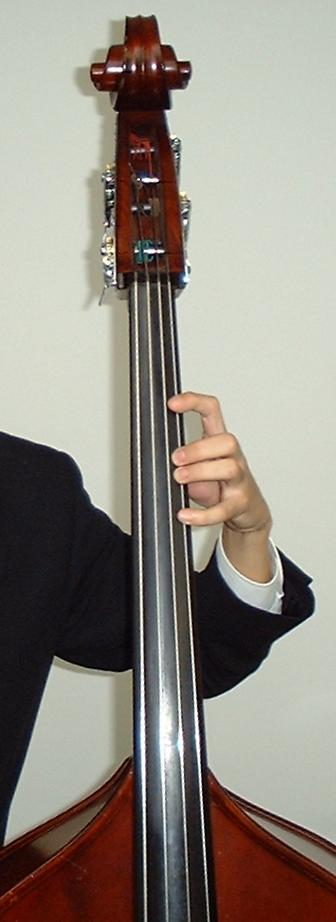
\includegraphics[height=7cm]{Pics/Position/1st_1.epsi}\\
{\small 図\thefigure : 第Iポジション\\}
\end{center}
\end{minipage}
\hfill
\begin{minipage}{90pt}
\addtocounter{figure}{1}
\begin{center}
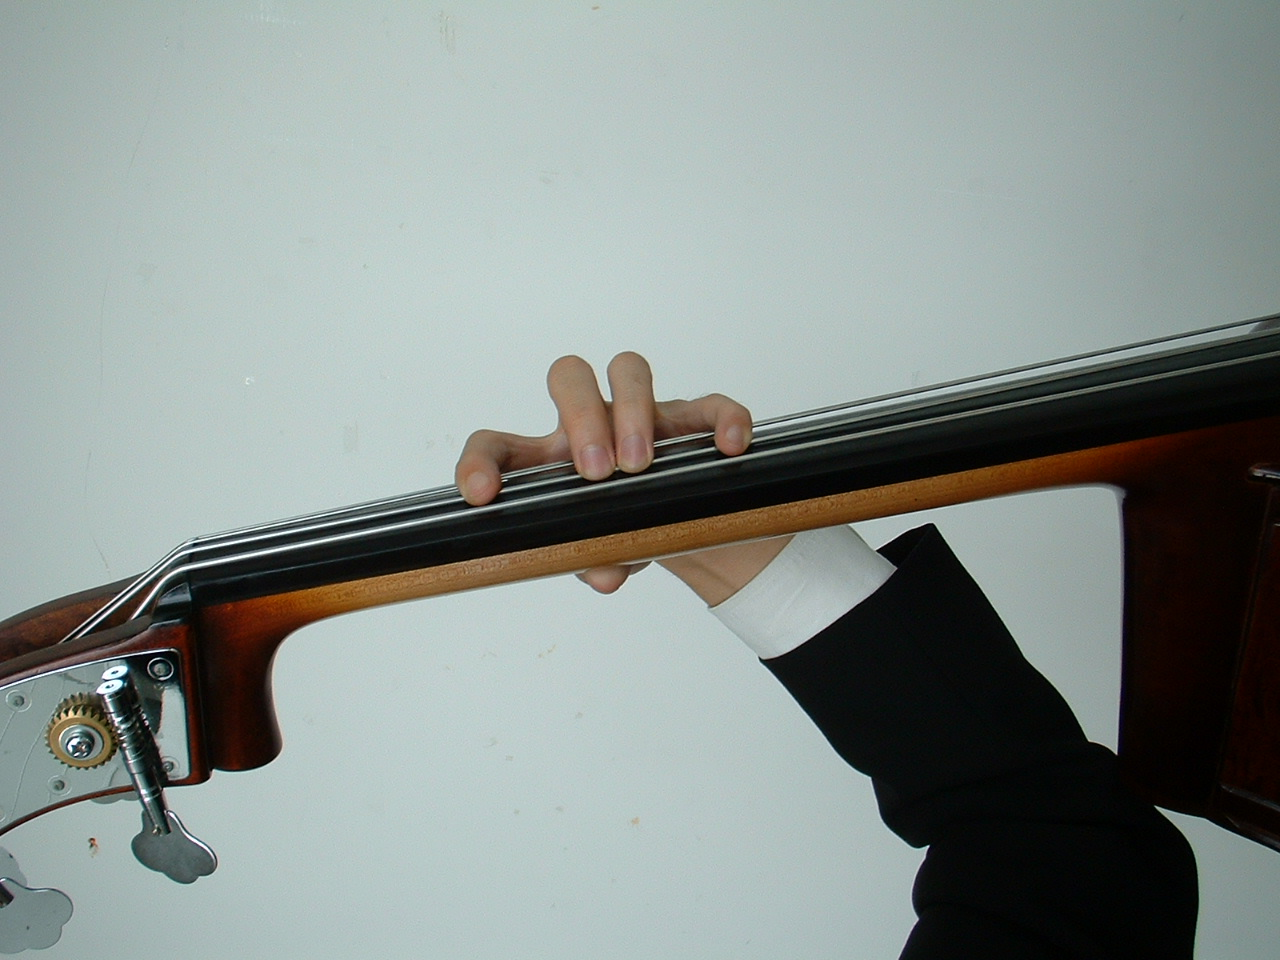
\includegraphics[height=7cm]{Pics/newphoto/1st.epsi}\\
{\small 図\thefigure : 奏者側から\\}
\end{center}
\end{minipage}
\end{flushleft}

\subsection{音階練習 \label{1st_scale}}
\begin{music}
\nostartrule
\parindent 0pt
\setclef1{\bass}  
\generalmeter{\meterC}
\generalsignature{2}    
\startpiece
\notes\zchar{19}{ニ長調(D-dur)音階}\enotes
\NOtes\zchar{14}{I}\ovbkt{!e}{5.5}{3}\zchar{6}{\bf 0}\ql{'D}\zchar{7}{\bf 1}\ql{E}\zchar{8}{\bf 4}\ql{F}\zchar{9}{\bf 0}\ql{G}\enotes
\bar
\NOtes\zchar{10}{\bf 1}\ql{!a}\zchar{11}{\bf 4}\ql{b}\zchar{18}{III}\ovbkt{'c}{3.5}{0}\zchar{12}{\bf 2}\ql{!c}\zchar{13}{\bf 4}\ql{d}\enotes
\bar
\NOtes\zchar{13}{\bf 4}\ql{d}\zchar{12}{\bf 2}\ql{c}\zchar{11}{\bf 4}\zchar{17}{I}\ovbkt{'b}{5.5}{-3}\ql{!b}\zchar{10}{\bf 1}\ql{a}\enotes
\bar
\NOtes\zchar{9}{\bf 0}\ql{'G}\zchar{8}{\bf 4}\ql{F}\zchar{7}{\bf 1}\ql{E}\zchar{6}{\bf 0}\ql{D}\enotes
\setdoublebar\endpiece
\setclef1{\bass}  
\generalmeter{\meterC}
\generalsignature{3}    
\startpiece
\notes\zchar{19}{イ長調(A-dur)音階}\enotes
\NOtes\zchar{14}{I}\zchar{9}{\bf 0}\ovbkt{!f}{5.5}{0}\qu{'A}\zchar{9}{\bf 1}\qu{B}\zchar{9}{\bf 4}\qu{C}\zchar{9}{\bf 0}\ql{D}\enotes
\bar
\NOtes\zchar{9}{\bf 1}\ql{'E}\zchar{9}{\bf 4}\ql{F}\zchar{15}{III}\ovbkt{!g}{3.5}{0}\zchar{9}{\bf 2}\ql{'G}\zchar{10}{\bf 4}\ql{!a}\enotes
\bar
\NOtes\zchar{10}{\bf 4}\ql{!a}\zchar{9}{\bf 2}\ql{'G}\zchar{9}{\bf 4}\zchar{14}{I}\ovbkt{!f}{5.5}{0}\ql{'F}\zchar{9}{\bf 1}\ql{E}\enotes
\bar
\NOtes\zchar{9}{\bf 0}\ql{'D}\zchar{9}{\bf 4}\qu{C}\zchar{9}{\bf 1}\qu{B}\zchar{9}{\bf 0}\qu{A}\enotes
\setdoublebar\endpiece
\setclef1{\bass}  
\generalmeter{\meterC}
\generalsignature{4}    
\startpiece
\notes\zchar{19}{ホ長調(E-dur)音階}\enotes
\NOtes\zchar{9}{\bf 0}\zchar{14}{I}\ovbkt{!f}{5.5}{0}\qu{E}\zchar{9}{\bf 1}\qu{F}\zchar{9}{\bf 4}\qu{G}\zchar{9}{\bf 0}\qu{'A}\enotes
\bar
\NOtes\zchar{9}{\bf 1}\qu{'B}\zchar{9}{\bf 4}\qu{C}\zchar{15}{III}\ovbkt{!g}{3.5}{0}\zchar{9}{\bf 2}\ql{'D}\zchar{9}{\bf 4}\ql{E}\enotes
\bar
\NOtes\zchar{9}{\bf 4}\ql{'E}\zchar{9}{\bf 2}\ql{D}\zchar{14}{I}\ovbkt{!f}{5.5}{0}\zchar{9}{\bf 4}\qu{'C}\zchar{9}{\bf 1}\qu{B}\enotes
\bar
\NOtes\zchar{9}{\bf 0}\qu{'A}\zchar{9}{\bf 4}\qu{!G}\zchar{9}{\bf 1}\qu{F}\zchar{9}{\bf 0}\qu{E}\enotes
\setdoublebar\endpiece
\end{music}


\subsection{第Iポジションで弾ける名曲}
\documentclass{jarticle}
\usepackage{musixdoc}
\startmuflex\makeindex

\begin{document}

\subsubsection*{�ե��: ����ʥ�ûĴ ��3�ھϤ��}
\begin{music}
\nostartrule
\setclef1{\bass}
\generalsignature{2}    
\generalmeter{\allabreve}
\parindent 0pt
\startbarno=268
\def\writebarno{\tenrm\the\barno\barnoadd}
\def\raisebarno{2\internote}
\def\shiftbarno{0.1\Interligne}
\systemnumbers
\startpiece\bigaccid
\notes\zchar{18}{\bf (Allegro non troppo)}\enotes
\Notes\ql{'F!a'FE}\enotes
\bar
\Notes\ql{'E!a'FD}\enotes
\bar
\Notes\ql{bcda}\enotes
\bar
\Notes\ql{a'FD}\qp\enotes
\bar
\Notes\qp\qu{'A!GF}\enotes
\bar
\Notes\hu{'BA}\enotes
\bar
\Notes\qp\ql{a'GF}\enotes
\bar
\Notes\hl{'D}\qu{C}\ql{F}\enotes
\bar
\Notes\ql{'F!a'FE}\enotes
\bar
\Notes\ql{'E!a'FD}\enotes
\bar
\Notes\qu{'BC}\ql{D}\qu{C}\enotes
\bar
\Notes\qu{'CA!F}\qp\enotes
\setdoublebar
\endpiece
\end{music}
\endmuflex
\end{document}

\documentclass{jarticle}
\usepackage{musixdoc}
\startmuflex\makeindex

\begin{document}

\subsubsection*{�ɥ����륶����: �������8�� ��ĹĴ ��4�ھϤ��}

\begin{music}
\nostartrule
\setclef1{\bass}
\generalsignature{1}    
\generalmeter{\meterfrac24}
\parindent 0pt
\startbarno=54
\def\writebarno{\tenrm\the\barno\barnoadd}
\def\raisebarno{2\internote}
\def\shiftbarno{0.1\Interligne}
\systemnumbers
\startpiece\bigaccid
\notes\zchar{18}{\bf (Allegro ma non troppo)}\enotes
\Notes\zchar{9}{arco}\zchar{-4}{\ff}\cl{'G}\ds\cl{!b}\ds\enotes
\bar
\NOtes\isluru{0}{d}\usfz{d}\hl{d}\enotes
\bar
\Notes\ibl{0}{c}{0}\tslur{0}{d}\qb{0}{d}\enotes
\notes\ibbl{0}{c}{0}\qb{0}{c}\tbbl{0}\tbl{0}\qb{0}{d}\enotes
\Notes\ibl{0}{e}{-2}\qb{0}{e}\tbl{0}\usfz{c}\isluru{0}{c}\qb{0}{c}\enotes
\bar
\Notes\ibl{0}{b}{0}\tslur{0}{c}\qb{0}{c}\enotes
\notes\ibbl{0}{b}{0}\qb{0}{b}\tbbl{0}\tbl{0}\qb{0}{c}\enotes
\Notes\ibl{0}{d}{-2}\qb{0}{d}\tbl{0}\isluru{0}{b}\usfz{b}\qb{0}{b}\enotes
\bar
\Notes\ibl{0}{a}{0}\tslur{0}{b}\qb{0}{b}\enotes
\notes\ibbl{0}{a}{0}\qb{0}{a}\tbbl{0}\tbl{0}\qb{0}{b}\enotes
\Notes\ibl{0}{c}{-2}\qb{0}{c}\tbl{0}\qb{0}{a}\enotes
\bar
\Notes\ibl{0}{'F}{3}\upz{E}\qb{0}{E}\tbl{0}\upz{!e}\qb{0}{e}\enotes
\Notes\ibl{0}{d}{-2}\upz{d}\qb{0}{d}\tbl{0}\upz{c}\qb{0}{c}\enotes
\bar
\Notes\ibl{0}{b}{0}\upz{b}\qb{0}{b}\tbl{0}\upz{b}\qb{0}{_b}\enotes
\Notes\ibl{0}{a}{1}\upz{a}\qb{0}{a}\tbl{0}\upz{b}\qb{0}{=b}\enotes
\bar
\Notes\ibl{0}{'G}{1}\upz{G}\qb{0}{G}\tbl{0}\upz{!a}\qb{0}{a}\enotes
\Notes\upz{'D}\cl{D}\ds\enotes
\leftrightrepeat
\Notes\zchar{-6}{\ff}\cl{'D}\ds\cl{E}\ds\enotes
\bar
\NOtes\zchar{-4}{\ppfftwenty fz}\qlp{'G}\enotes
\notes\cl{'F}\enotes
\bar
\Notes\cl{'E}\ds\cl{!b}\ds\enotes
\bar
\NOtes\zchar{-4}{\ppfftwenty fz}\qlp{d}\enotes
\notes\cl{^c}\enotes
\bar
\Notes\loffset{0.5}{\zchar{-4}{\ppfftwenty pi\'{u} f}}\usf{b}\ql{b}\usf{a}\ql{a}\enotes
\bar
\Notes\ibl{0}{'G}{-2}\usf{!a}\upz{'G}\qb{0}{G}\upz{F}\qb{0}{F}\upz{E}\qb{0}{E}\tbl{0}\upz{D}\qb{0}{D}\enotes
\bar
\Notes\ibu{0}{'C}{0}\qb{0}{C}\qb{0}{A}\qb{0}{B}\tbu{0}\qb{0}{C}\enotes
\bar
\Notes\ibl{0}{'D}{0}\qb{0}{D}\enotes
\notes\ibbl{0}{D}{0}\qb{0}{!d}\tbbl{0}\tbl{0}\qb{0}{'D}\enotes
\Notes\cl{'G}\ds\enotes
\setrightrepeat\endpiece
\end{music}

\endmuflex
\end{document}

\subsubsection*{チャイコフスキー: 弦楽セレナーデ ハ長調 第1楽章 「ソナチナ形式の小品」より}

\begin{music}
\nostartrule
\setclef1{\bass}
\generalsignature{0}    
\generalmeter{\meterfrac68}
\parindent 0pt
\def\writebarno{\tenrm\the\barno\barnoadd}
\def\raisebarno{2\internote}
\def\shiftbarno{0.1\Interligne}
\systemnumbers
\startpiece\bigaccid
\notes\zchar{22}{\bf Andante non troppo}\enotes
\NOtes\zchar{-4}{\f}\zchar{-8}{III}\zchar{14}{\downbow}\zchar{12}{\bf 4}\usf{a}\qlp{a}\zchar{11}{\bf 1}\usf{'G}\qlp{G}\enotes
\bar
\NOtes\zchar{-5}{\it sempre marcatissimo}\zchar{14}{\downbow}\zchar{12}{\bf 2}\zchar{-9}{I}\usf{'G}\qlp{F}\enotes
\notes\ibl{0}{'E}{0}\zchar{12}{\upbow}\qb{0}{EF}\tbl{0}\qb{0}{E}\enotes
\bar
\NOtes\zchar{-9}{II}\zchar{6}{\bf 4}\qlp{'D}\zchar{9}{\bf 4}\qlp{G}\enotes
\bar
\NOtes\zchar{-5}{III}\zchar{9}{\bf 2}\qlp{'^G}\enotes
\notes\ibl{0}{!a}{-3}\qb{0}{a=!'G}\tbl{0}\zchar{-5}{I}\zchar{9}{\bf 2}\qb{0}{F}\enotes
\bar
\NOtes\zchar{-6}{\icresc}\zchar{9}{\downbow}\qlp{'E}\enotes
\Notes\xtuplet{2}{'E}\ibl{0}{D}{1}\zchar{9}{\upbow}\zchar{6}{\bf 0}\qb{0}{D}\tbl{0}\zchar{10}{\downbow}\zchar{7}{\bf 1}\qb{0}{!'E}\enotes
\bar
\NOtes\isluru{0}{'F}\zchar{9}{\upbow}\qlp{F}\enotes
\Notes\isluru{1}{'G}\zchar{16}{\downbow}\zchar{14}{\bf 4}\zchar{-4}{II}\ql{G}\enotes
\notes\ibbl{0}{'G}{-6}\tslur{0}{G}\tslur{1}{G}\qb{0}{G}\zchar{-6}{\tcresc}\tbbl{0}\tbl{0}\zchar{-5}{\ff}\zchar{13}{\downbow}\zchar{11}{\bf 1}\qb{0}{C}\enotes
\alaligne 
\NOtes\zchar{-5}{\ppfftwenty sf}\zchar{10}{\upbow}\qup{'C}\zchar{-5}{\ppfftwenty sf}\islurd{0}{C}\zchar{10}{\downbow}\qup{C}\enotes
\generalmeter{\meterfrac24}\changecontext 
\notes\ibbl{0}{'C}{3}\tslur{0}{C}\qb{0}{C}\zchar{14}{\upbow}\zchar{11}{\bf 2}\usf{!'G}\zchar{-9}{I}\qb{0}{C}\zchar{14}{\downbow}\zchar{11}{\bf 0}\usf{G}\qb{0}{D}\zchar{14}{\upbow}\zchar{11}{\bf 1}\usf{G}\qb{0}{E}\zchar{11}{\bf 2}\usf{G}\qb{0}{F}\zchar{11}{\bf 0}\usf{G}\qb{0}{G}\zchar{12}{\bf 1}\usf{'A}\qb{0}{A}\tbbl{0}\tbl{0}\zchar{-5}{II}\zchar{13}{\bf 2}\usf{!b}\qb{0}{!b}\enotes
\generalmeter{\meterfrac68}\changecontext
\NOtes\zchar{-7}{\ff \ \it marcatissimo}\zchar{14}{\downbow}\zchar{12}{\bf 4}\qlp{cb}\enotes
\bar
\NOtes\zchar{-5}{I}\zchar{12}{\downbow}\zchar{10}{\bf 1}\qlp{a}\enotes
\notes\ibl{0}{'G}{2}\zchar{12}{\upbow}\zchar{9}{\bf 0}\qb{0}{G!a}\tbl{0}\zchar{-5}{II}\zchar{12}{\bf 4}\qb{0}{c}\enotes
\bar
\NOtes\isluru{0}{'G}\zchar{12}{\downbow}\zchar{9}{\bf 4}\qlp{G}\enotes
\Notes\tslur{0}{'G}\ql{G}\zchar{10}{\upbow}\cl{F}\enotes
\bar
\NOtes\zchar{-5}{I}\zchar{9}{\bf 1}\qlp{'E}\enotes
\notes\ibl0{'E}{1}\qb0{EE}\tbl0\qb0{!a}\enotes
\bar
\NOtes\zchar{-5}{II}\zchar{11}{\downbow}\zchar{9}{\bf 4}\qlp{'G}\enotes
\Notes\xtuplet{2}{'E}\ibl{0}{F}{-2}\zchar{-6}{I}\zchar{10}{\upbow}\zchar{8}{\bf 2}\qb{0}{F}\tbl{0}\zchar{9}{\downbow}\qb0{E}\enotes
\bar
\NOtes\zchar{-6}{II}\zchar{9}{\upbow}\zchar{7}{\bf 4}\qlp{'D}\enotes
\Notes\isluru{0}{'G}\zchar{11}{\downbow}\ql{G}\enotes
\notes\ibbl{0}{'G}{-6}\tslur{0}{G}\qb{0}{G}\tbbl{0}\tbl{0}\zchar{9}{\downbow}\qb{0}{C}\enotes
\bar
\NOtes\zchar{10}{\upbow}\qup{'C}\enotes
\notes\zchar{-5}{\fff}\zchar{12}{\downbow}\cl{!c}\ds\ds\enotes
\mulooseness=0
\setdoublebar\endpiece
\end{music}

%\subsubsection*{シューベルト: ピアノ五重奏曲「ます」 第4楽章 第3変奏}

\begin{music}
\nostartrule
\startbarno=61
\def\writebarno{\tenrm\the\barno\barnoadd}
\def\raisebarno{2\internote}
\def\shiftbarno{0.1\Interligne}
\systemnumbers
\setclef1{\bass}
\generalsignature{2}    
\generalmeter{\meterfrac24}
\parindent 0pt
\startpiece\bigaccid
\notes\zchar{16}{\bf Var. III}\enotes
\Notes\zchar{-5}{II}\zchar{-8}{\p}\zchar{11}{\upbow}\zchar{8}{\bf 4}\lpz{'A}\cu{A}\enotes
\leftrepeat
\Notes\ibl{0}{'D}{0}\zchar{10}{\downbow}\zchar{8}{\bf 4}\upz{D}\qb{0}{D}\zchar{8}{\upbow}\upz{D}\qb{0}{D}\upz{F}\qb{0}{F}\tbl{0}\upz{F}\qb{0}{F}\enotes
\bar
\Notes\qu{'D}\qu{A}\enotes
\barno=62
\bar
\Notes\ibu{0}{'A}{0}\islurd{0}{A}\zchar{8}{\downbow}\qbp{0}{A}\tbbu{0}\tbu{0}\tslur{0}{!G}\lpz{'A}\qb{0}{A}\enotes
\Notes\ibbu{0}{'E}{-2}\islurd{0}{E}\zchar{-5}{III}\zchar{16}{\upbow}\zchar{13}{\bf 4}\qbp{0}{E}\tbbbu{0}\zchar{13}{\bf 1}\qb{0}{D}\zchar{-5}{I}\zchar{12}{\bf 4}\qbp{0}{C}\tbbbu{0}\tbbu{0}\tbu{0}\tslur{0}{B}\zchar{12}{\bf 1}\qb{0}{B}\enotes
\bar
\Notes\zchar{-4}{II}\zchar{11}{\downbow}\zchar{8}{\bf 4}\qu{'A}\enotes
\notes\ds\zchar{8}{\upbow}\cu{'A}\enotes
\bar
\Notes\ibl{0}{'D}{0}\zchar{8}{\downbow}\upz{D}\qb{0}{D}\zchar{8}{\upbow}\upz{D}\qb{0}{D}\upz{F}\qb{0}{F}\tbl{0}\upz{F}\qb{0}{F}\enotes
\bar
\Notes\ql{'D}\ibu{0}{C}{4}\islurd{0}{!G}\lpz{'A}\qb{0}{A}\tbu{0}\tslur{0}{C}\zchar{-4}{III}\lpz{D}\zchar{12}{\bf 1}\qb{0}{D}\enotes
\bar
\Notes\zchar{10}{\downbow}\zchar{8}{\bf 4}\cl{'E}\ds\zchar{8}{\upbow}\cl{E}\ds\enotes
\bar
\Notes\zchar{8}{\downbow}\qup{'A}\zchar{8}{\upbow}\cu{A}\enotes
\rightrepeat
\Notes\ibu{0}{'C}{0}\zchar{-5}{II}\zchar{12}{\downbow}\zchar{10}{\bf 2}\lpz{C}\qb{0}{C}\tbu{0}\zchar{10}{\upbow}\lpz{C}\qb{0}{C}\enotes
\notes\ibbu{0}{'B}{0}\islurd{0}{D}\zchar{13}{\downbow}\zchar{11}{\bf 4}\qb{0}{D}\zchar{11}{\bf 2}\qb{0}{C}\zchar{-5}{I}\zchar{11}{\bf 1}\qb{0}{B}\tbbu{0}\tbu{0}\tslur{0}{C}\zchar{-5}{II}\zchar{11}{\bf 2}\qb{0}{C}\enotes
\bar
\Notes\islurd{0}{'D}\zchar{13}{\upbow}\zchar{10}{\bf 4}\qu{D}\tslur{0}{A}\zchar{8}{\bf 4}\cu{A}\zchar{13}{\upbow}\zchar{10}{\bf 4}\cu{D}\enotes
\bar
\Notes\ibu{0}{'C}{0}\lpz{C}\qb{0}{C}\tbu{0}\lpz{C}\qb{0}{C}\enotes
\notes\ibbl{0}{'E}{0}\isluru{0}{E}\qb{0}{C}\midslur{3}\qb{0}{G}\zchar{-7}{I}\zchar{10}{\bf 1}\qb{0}{E}\tbbl{0}\tbl{0}\tslur{0}{C}\zchar{-7}{II}\zchar{9}{\bf 2}\qb{0}{C}\enotes
\bar
\Notes\islurd{0}{'D}\zchar{13}{\upbow}\zchar{10}{\bf 4}\qu{D}\tslur{0}{`D}\cu{D}\zchar{10}{\upbow}\cu{'D}\enotes
\bar
\Notes\ibu{0}{'B}{2}\zchar{-5}{III}\zchar{12}{\downbow}\zchar{10}{\bf 4}\qb{0}{B}\zchar{10}{\upbow}\qb{0}{BB}\tbu{0}\zchar{11}{\bf 1}\qb{0}{D}\enotes
\bar
\Notes\islurd{0}{'D}\zchar{11}{\downbow}\lsf{A}\qu{D}\tslur{0}{A}\zchar{8}{\bf 1}\cu{A}\zchar{9}{\upbow}\cu{A}\enotes
\bar
\Notes\ibu{0}{'A}{0}\zchar{8}{\downbow}\qbp{0}{A}\tbbu{0}\tbu{0}\zchar{8}{\upbow}\qb{0}{A}\ibu{0}{E}{-4}\zchar{14}{\downbow}\zchar{12}{\bf 4}\qb{0}{E}\tbu{0}\zchar{-5}{II}\zchar{14}{\upbow}\zchar{11}{\bf 2}\qb{0}{C}\enotes
\bar
\Notes\islurd{0}{'D}\zchar{11}{\downbow}\qu{D}\tslur{0}{`D}\cu{D}\zchar{10}{\upbow}\cu{'D}\enotes
\bar
\Notes\ibu{0}{'B}{2}\zchar{-5}{III}\zchar{10}{\bf 4}\qb{0}{BBB}\tbu{0}\zchar{12}{\bf 1}\qb{0}{D}\enotes
\bar
\Notes\islurd{0}{'D}\usf{!b}\qu{'D}\tslur{0}{A}\zchar{8}{\bf 1}\cu{A}\cu{A}\enotes
\bar
\Notes\ibu{0}{'A}{0}\qbp{0}{A}\tbbu{0}\tbu{0}\qb{0}{A}\ibu{0}{E}{-4}\zchar{12}{\bf 4}\qb{0}{E}\tbu{0}\zchar{-5}{II}\zchar{12}{\bf 2}\qb{0}{C}\enotes
\bar
\Notes\qlp{'D}\enotes
\mulooseness=0
\setdoublebar\endpiece
\end{music}

